
\setcounter{chapter}{4}
\chapter{Evaluation}
\minitoc %insert la minitoc
\graphicspath{{Chapitre5/figures/}}

%\DoPToC
%==============================================================================
\pagestyle{fancy}
\fancyhf{}
\fancyhead[R]{\bfseries\rightmark}
\fancyfoot[R]{\thepage}
\renewcommand{\headrulewidth}{0.5pt}
\renewcommand{\footrulewidth}{0pt}
\renewcommand{\chaptermark}[1]{\markboth{{\chaptername~\thechapter. #1 }}{}}
\renewcommand{\sectionmark}[1]{\markright{\thechapter.\thesection~ #1}}

\begin{spacing}{1.2}

%==============================================================================
\section*{Introduction}
This chapter presents a comprehensive evaluation of the LLM-powered best practices enforcement system that drove the architectural decisions described in Chapter 3 and the implementation choices detailed in Chapter 4. The evaluation focuses on comparing three distinct agent architectures to determine the optimal approach for production deployment, analyzing their performance across accuracy, latency, and cost metrics.

The results presented in this chapter directly informed the design decisions and implementation strategies outlined in previous chapters, demonstrating how data-driven evaluation shaped the final system architecture.

\section{Evaluation Methodology}

\subsection{Test Suite Framework}
We created a comprehensive suite of 12 test cases covering a wide range of scenarios to evaluate the three agent architectures. This test suite provides diverse complexity levels and violation patterns to ensure robust evaluation across different use cases.

\subsection{LLM-as-a-Judge Evaluation Approach}
The most novel aspect of our evaluation framework is the "LLM-as-a-Judge" methodology. A significant challenge in testing LLMs is the inherent variability in their outputs, making simple text comparison methods too brittle for reliable assessment.

Our solution employs another LLM as an impartial judge that semantically compares the agent's response to the ideal answer. This approach understands the meaning behind the words rather than requiring exact text matches, providing a much more realistic and robust measure of quality.

\subsection{Key Metrics}
With this evaluation framework in place, we track three critical metrics that determine system viability:

\begin{itemize}
    \item \textbf{Accuracy}: Determined by our LLM judge through semantic comparison
    \item \textbf{Latency}: Processing speed measured in seconds
    \item \textbf{Cost}: Token consumption and associated computational costs
\end{itemize}

\section{Agent Architecture Comparison}

\subsection{Architecture Variants}
Three distinct agent architectures were implemented and evaluated to inform the design decisions presented in Chapter 3. These architectures represent different approaches to balancing performance, reliability, and resource efficiency:

\begin{itemize}
    \item \textbf{Sequential Executable}: Processes violations one by one, ensuring deterministic execution and maximum reliability. This approach was evaluated to establish a baseline for reliability and consistency.
    \item \textbf{Parallel Executable}: Processes all violations concurrently using asyncio.gather, maximizing throughput through parallelization. This architecture was tested to assess the potential performance gains and associated risks.
    \item \textbf{ReAct Agent}: Uses a ReAct loop with multi-step reasoning, representing the traditional agent paradigm. This approach was included to evaluate the effectiveness of dynamic reasoning versus predefined execution patterns.
\end{itemize}

The evaluation of these three architectures directly informed the hybrid approach described in Chapter 3, where we ultimately selected the parallel executable architecture with concurrency limiting based on the performance and reliability data presented in this chapter.

\section{Performance Analysis Results}

\subsection{Single-Violation File Analysis}
For a simple file with only one violation (TC8\_PROPS\_MISSING\_EXPORT), the performance differences are stark:

\begin{table}[H]
\centering
\caption{Single-Violation File Performance Comparison}
\footnotesize
\begin{tabular}{|l|c|c|c|}
\hline 
\textbf{Architecture} & \textbf{Latency} & \textbf{Input Tokens} & \textbf{Output Tokens} \\
\hline 
Parallel Executable & 4.1s & 5,157 & 331 \\
\hline
Sequential Executable & 6.1s & 5,157 & 331 \\
\hline
ReAct Agent & 15.3s & 37,989 & 1,523 \\
\hline
\end{tabular}
\label{tab:single_violation_performance}
\end{table}

\textbf{Key Takeaways:}
\begin{itemize}
    \item \textbf{Parallel vs. Sequential}: For a simple case, the overhead of asyncio.gather is negligible, making the parallel agent about 33\% faster than the sequential one. Token usage is identical.
    \item \textbf{Executable vs. ReAct}: The executable agents are vastly more efficient. The ReAct agent is ~2.7x slower than the sequential agent and uses ~7.4x more input tokens to solve the same simple problem.
\end{itemize}

\subsection{Full Evaluation Suite Analysis (12 Cases)}
When scaling up to the full test suite, the reliability of the parallel agent becomes the central issue. The following charts illustrate the comprehensive performance comparison across all 12 test cases:

\begin{figure}[H]
\centering
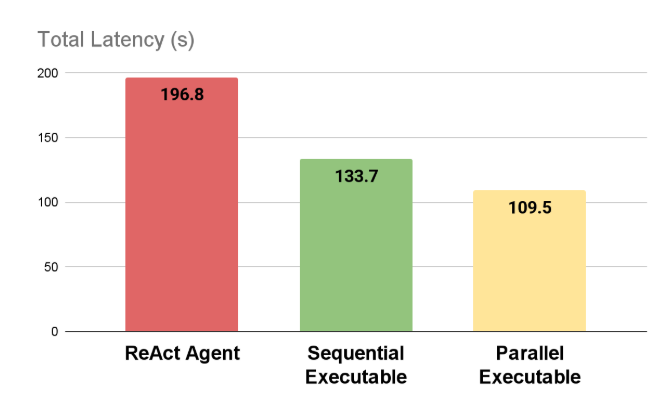
\includegraphics[scale=0.5]{images/latency.png}
\caption{Latency Performance Comparison Across 12 Test Cases}
\label{fig:latency_comparison}
\end{figure}

\textbf{Latency Performance (Chart 1):} The latency chart clearly demonstrates the parallel agent's speed advantage, completing the entire test suite about 22\% faster than the sequential agent. However, this performance comes with a critical caveat - the parallel agent's success is conditional and depends on the total number of concurrent API calls.

\begin{figure}[H]
\centering
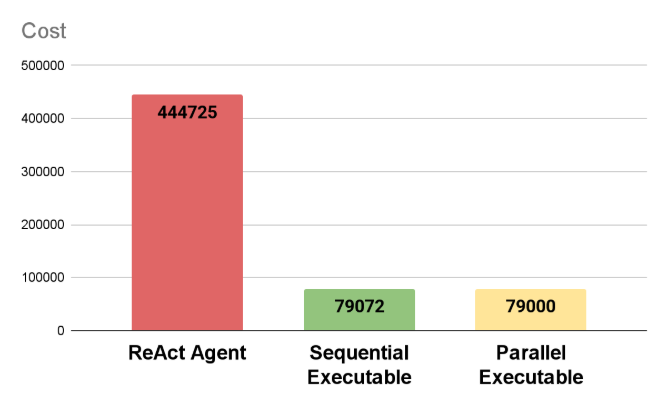
\includegraphics[scale=0.5]{images/cost.png}
\caption{Cost Analysis Across 12 Test Cases}
\label{fig:cost_comparison}
\end{figure}

\textbf{Cost Analysis (Chart 2):} The cost comparison reveals the ReAct agent's fundamental inefficiency, consuming nearly six times more tokens than the executable agents. This massive cost differential makes the ReAct approach non-viable for production deployment, effectively eliminating it from consideration.

\begin{figure}[H]
\centering
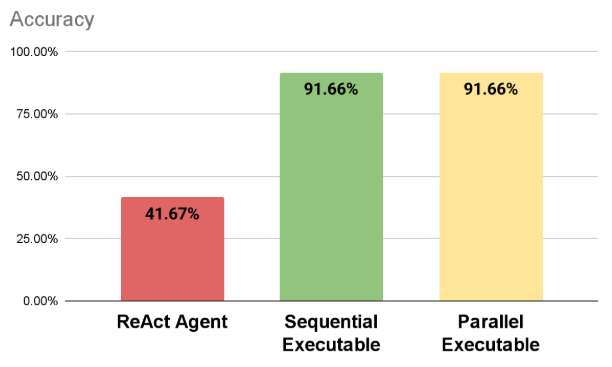
\includegraphics[scale=0.5]{images/accuracy.png}
\caption{Accuracy Performance Across 12 Test Cases}
\label{fig:accuracy_comparison}
\end{figure}

\textbf{Accuracy Performance (Chart 3):} While both executable agents achieve identical accuracy rates of 91.66\%, the parallel agent's reliability becomes the deciding factor. The sequential agent maintains 100\% reliability across all test runs, while the parallel agent suffers from OverLimitException and DEADLINE\_EXCEEDED errors under heavy load.

\textbf{Key Takeaways:}
\begin{itemize}
    \item \textbf{The Reliability Flaw}: While the parallel agent was ~22\% faster in its successful run, it has also been observed to crash with OverLimitException when encountering files with many violations. Its success is conditional and depends on the total number of concurrent API calls, which can easily exceed service quotas.
    \item \textbf{The Stability of Sequential}: The sequential agent is the only architecture that has proven to be 100\% reliable across all test runs.
    \item \textbf{ReAct's Inefficiency}: The ReAct agent remains non-viable due to its low accuracy and extremely high cost.
\end{itemize}

\subsection{Detailed Performance Analysis}
Let's examine the data we found when comparing our three candidates:

\textbf{Latency Analysis}: If this were just about being fast, the parallel agent would be the clear winner. It had the lowest latency, completing the entire test suite about 22\% faster than the sequential one. But as we'll see, the lowest latency isn't the whole story.

\textbf{Cost Analysis}: This is where the ReAct agent fell apart. Because of its ReAct loop—where it has to 'think' step-by-step about what to do next—it consumed a massive number of tokens. It cost nearly six times more to do the exact same job. That incredible inefficiency made it non-viable, so right away, we knew ReAct was out. This narrowed our choice down to the two executable models.

\textbf{Accuracy Analysis}: Looking at the results, the Sequential agent was very accurate, with a solid 91.7\% success rate. And the Parallel agent appears to match it perfectly. But there's a critical catch. That high accuracy is only for the runs where it didn't crash. We discovered that under heavy load, its fully parallel nature would cause it to fail completely. And the agent with the lowest latency is useless if it's not reliable.

So, the data left us with a clear puzzle: ReAct was too expensive. Sequential was reliable but had higher latency. And Parallel had the lowest latency but was critically unstable. The question became: how could we get the speed we wanted, without all the risk?

\section{Final Recommendation}

\subsection{Implement the Parallel Agent with Concurrency Limiting}
The core decision comes down to a trade-off between the parallel agent's raw speed and its reliability under load. Our findings show that while the fully parallel agent is the fastest in simple cases, it is prone to critical failures when processing files with many violations.

This evaluation directly drove the implementation strategy described in Chapter 4, where we implemented the parallel executable architecture with semaphore-based concurrency control to address the reliability issues identified in our testing.

The most recent test runs surfaced a DEADLINE\_EXCEEDED error. This occurs because flooding the backend with too many simultaneous requests overwhelms the service, preventing it from responding before the client-side timeout is reached. This is a more insidious failure than a simple quota error (OverLimitException) because it points to systemic overload. 

For a production tool, predictability and stability are paramount. A user encountering a hard error is a significantly worse experience than waiting a few extra seconds for a guaranteed result.

Therefore, the recommendation is to keep the parallel architecture but control its concurrency. By using a semaphore to limit the number of in-flight requests, we can retain most of the performance gains of parallelism while ensuring the agent remains stable and reliable, even under heavy load.

This approach gives us the best of both worlds: the speed of parallelism and the reliability of a sequential process. 

\section*{Conclusion}
This chapter presented a comprehensive evaluation of three agent architectures for the LLM-powered best practices enforcement system. Through our novel "LLM-as-a-Judge" evaluation methodology and comprehensive 12-test-case suite, we demonstrated that the parallel executable agent with concurrency limiting provides the optimal balance between performance and reliability.

The evaluation revealed that while the ReAct agent was eliminated due to its excessive cost and low accuracy, the choice between sequential and parallel executable agents required careful consideration of the reliability-speed trade-off. Our final recommendation of implementing the parallel agent with concurrency limiting achieves the best of both worlds: the speed of parallelism and the reliability of sequential processing.

This data-driven evaluation process directly informed the architectural decisions presented in Chapter 3 and guided the implementation strategies detailed in Chapter 4. The systematic comparison of agent architectures, performance analysis, and reliability assessment provided the empirical foundation for selecting the optimal approach, ensuring that design choices were based on concrete evidence rather than assumptions. This evaluation methodology demonstrates how rigorous testing and analysis can drive effective system design and implementation decisions.

%==============================================================================
\end{spacing}
